% !TeX root = ../../main.tex
% Add the above to each chapter to make compiling the PDF easier in some editors.

\chapter{Introduction}\label{chapter:introduction}

Reinforcement learning \textbf{(RL)} is an area of machine learning (Figure~\ref{fig:rl_2}) inspired by behaviorist psychology and intersect between different fields including neuroscience, psychology, mathematics and economics as shown in Figure~\ref{fig:rl_1}. It has revolutionized our understanding of learning in the brain over the last 20 years. Unlike other machine learning approaches, that are dependent on \textit{pre-collected data}, RL allows an agent to take actions to observe and interact with an environment to maximize total rewards towards achieving specific goals.

\begin{figure}[!htb]
	\centering
	\begin{subfigure}[b]{0.4\textwidth}
		\centering
		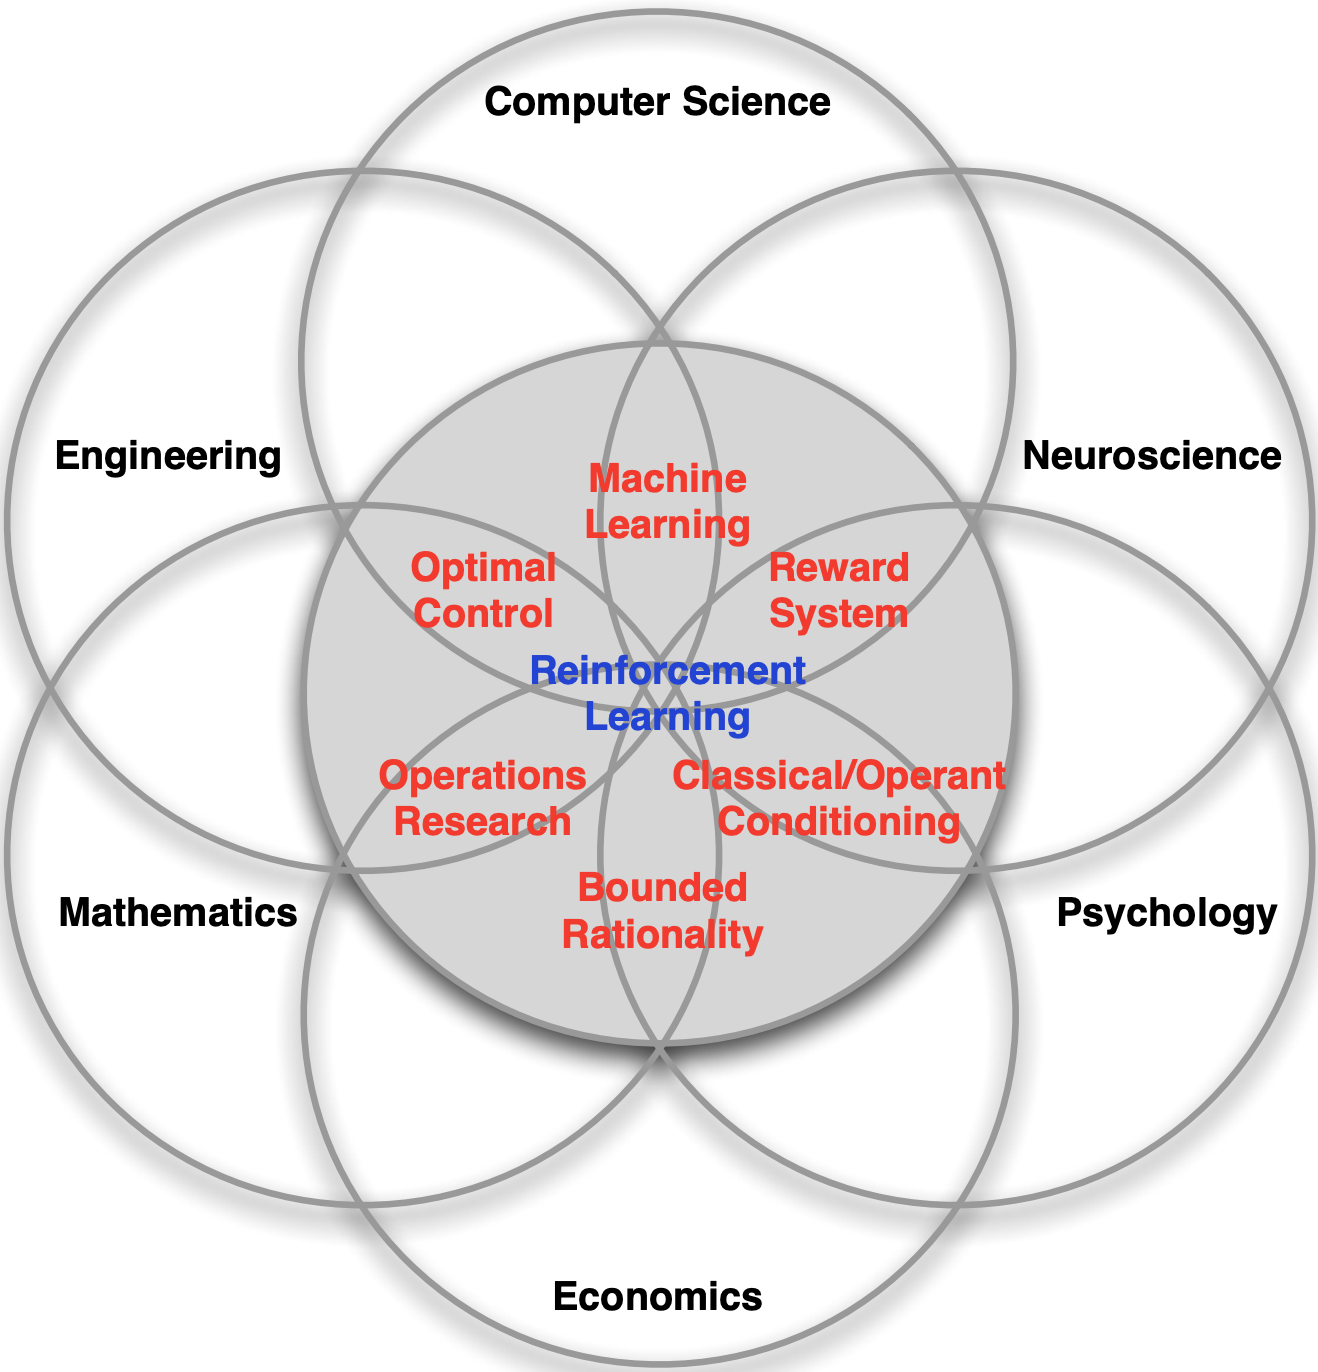
\includegraphics[width=1.1\textwidth]{figures/rl/rl_1.png}
		\caption{Faces of Reinforcement Learning}
		\label{fig:rl_1}
	\end{subfigure}
	\hfill
	\begin{subfigure}[b]{0.4\textwidth}
		\centering
		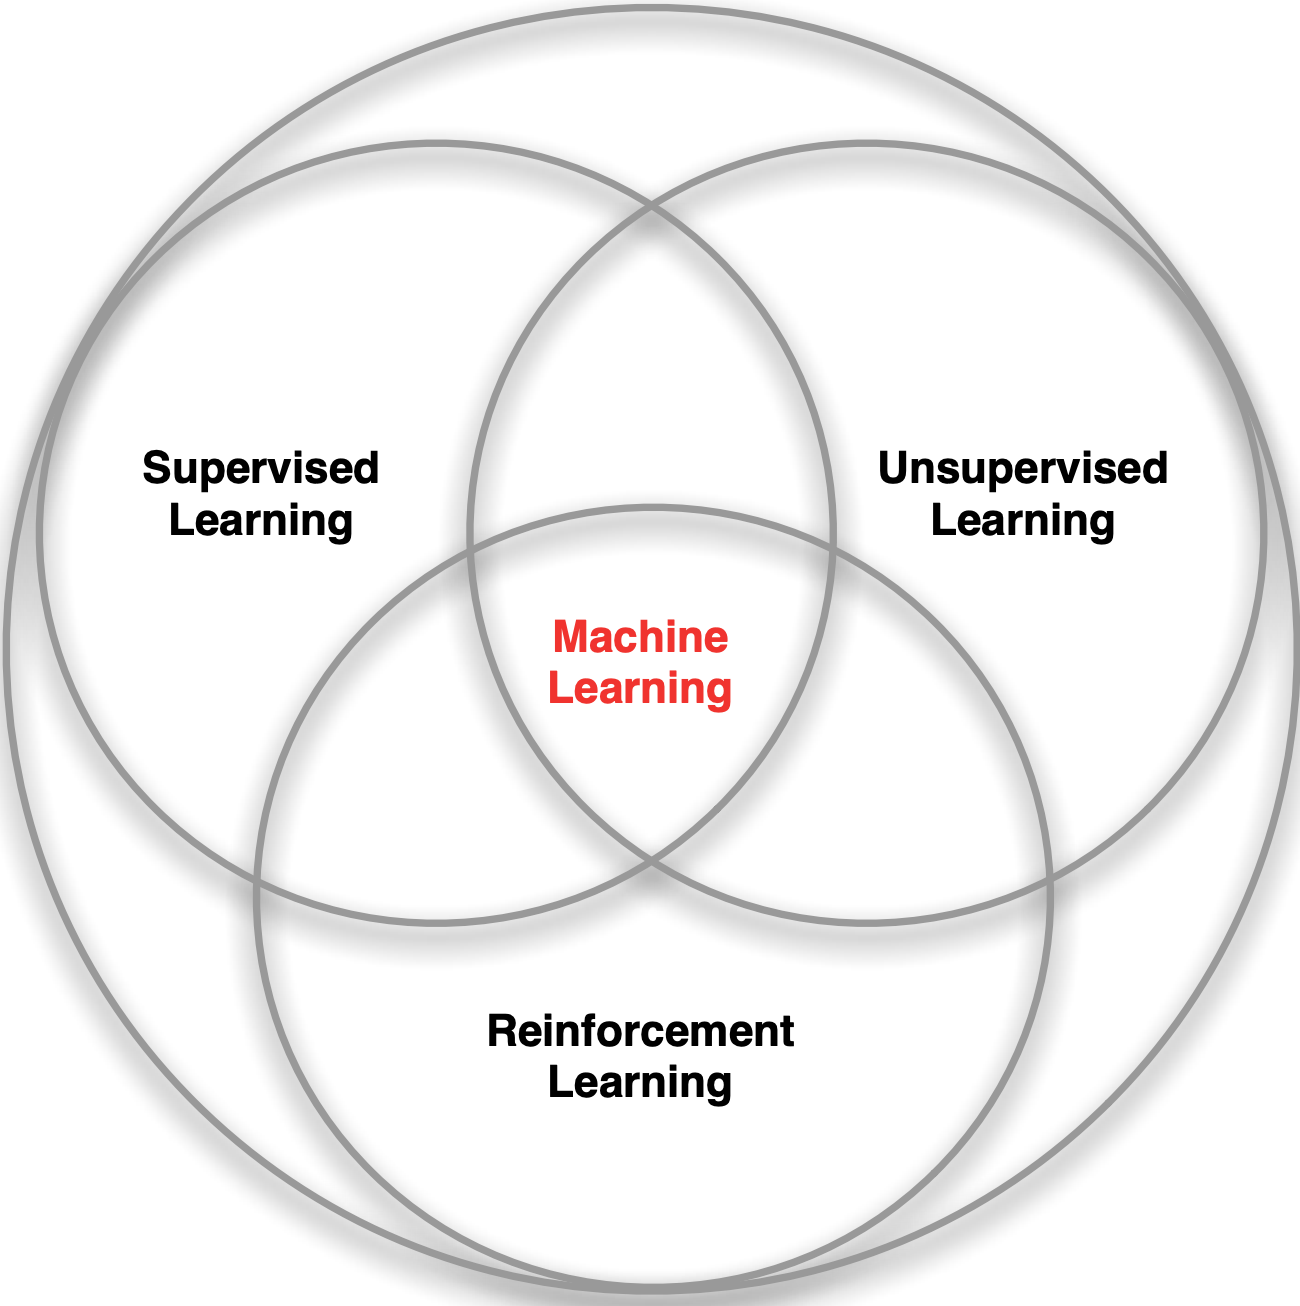
\includegraphics[width=1.1\textwidth]{figures/rl/rl_2.png}
		\caption{Branches of Machine Learning}
		\label{fig:rl_2}
	\end{subfigure}
	\hfill
	\caption[General Overview of Reinforcement Learning]{General Overview of Reinforcement Learning\protect\footnotemark}
	\label{fig:rl}
\end{figure}

\footnotetext{The Figures are from Advanced Deep Learning and Reinforcement Learning Course (COMPGI22) taught at \href{http://www.cs.ucl.ac.uk}{UCL} in partnership with \href{http://www.deepmind.com}{DeepMind}}


RL combined with deep learning offers a promising path within the study of intelligent systems. It is considered as \textit{a step towards achieving Artificial General Intelligence}, which mimics the human's ability to learn from its own experiences. It is best applied to situations where algorithms have to decide according to their environment.

Artificial General Intelligence \textbf{(AGI)} is a type of \textit{\textbf{meta-learning}} introducing one concept where a machine can successfully understand, learn and perform any intellectual task that a human being can and the ability to learn multiple tasks. This allows the machine to \textit{learn how to learn and generalize it to acquire new skills, the way humans do}. Hence, AGI focuses on the study of systems that can perform tasks successfully across different problem domains. Most of the current ``conventional'' artificial intelligence (AI) systems are domain-specific. General problem-solving ability is one that humans naturally exhibit along with decision making under uncertainty, which provides a generalization to facilitates broad situation inference. RL may pave one way for a contribution towards building systems that will eventually exhibit human-level intelligence.

Over the past few years, RL approaches have many interesting applications and advancements which achieved remarkable results in many areas. Starting from playing atari games and achieving human-level performance~\parencite{mnih2015human} to defeating champions of chess, shogi and Go~\footnote{\textit{In The game of Go, The number of possible configurations of the board is more than the number of atoms in the universe}} with \textbf{Deepmind's AlphaGo Zero}~\parencite{silver2017mastering}. This was followed by defeating the world's top players in the game of DOTA 2~\footnote{\textit{DOTA 2: a real-time strategy game, one of the most popular and complex esports games in the world which has an infinite number of states and gameplay}} with \textbf{OpenAI FIVE}\textsuperscript{\ref{alhpa_five}}. Moreover, RL have been used for complex tasks and sequential decision making in unknown environments which is very useful for complex applications and fields like \textit{robotics}~\parencite{kober2013reinforcement, levine2016end, gu2017deep, singh2019end}, \textit{autonomous driving}~\parencite{sallab2017deep, xu2018zero}, \textit{web system configurations and telecommunication}~\parencite{bu2009reinforcement}, \textit{computer clusters resources management}~\parencite{mao2016resource}, \textit{traffic light control}~\parencite{arel2010reinforcement}, and \textit{chemistry}~\parencite{zhou2017optimizing}.

\section{Motivation}

RL has achieved groundbreaking results leading the way to some of the best intelligent systems we could ever have. However, the current techniques and algorithms deal with learning to continuously operate within an uncertain environment based on delayed and limited feedback. This requires a huge amount of training data to be able to learn a policy \textit{(a mapping from the state of the environment to a choice of action)} that yields effective performance over time.

% Modify the sentence
Usually the training data get collected when the agent starts with no prior knowledge of the environment and collect experience through interacting with the environment. This still takes time in rendering, receiving the states from the environment, collect and store the data to be passed for the algorithm to update and enhance the agent performance. This training process might take many hours, days or even weeks for some complex algorithms and environment systems. Nevertheless, it requires an enormous amount of computing power to achieve the desired results. 

% Modify the sentence
Following in Figure~\ref{fig:zero_and_five}, two examples of the most successful and breakthrough advancements in RL field. We used these example to demonstrate the training time and huge computation power used in the training process.

\textbf{Deepmind's AlphaZero}~\parencite{silver2017mastering} starts learning by playing games against itself starting from completely random play. The neural network in AlphaGo Zero is trained from games of self-play by a novel reinforcement learning algorithm along with Monte-Carlo Tree Search (MCTS). AlphaGo Zero used a single machine with \textit{4 tensor processing units (TPUs)}, in contrast with AlphaGo that was distributed over many machines and used \textit{48 TPUs}. The training still took \textbf{21 days} to surpasses AlphaGo Master and \textbf{40 days} to surpass all other versions of AlphaGo as shown in the following Figure~\ref{fig:alphago_train}.

% GPU + CPU | Full Text
\textbf{OpenAI FIVE}~\parencite{OpenAI_dota} plays 180 years worth of games against itself every day, learning via self-play. It trains using a scaled-up version of Proximal Policy Optimization (PPO), shown in Figure~\ref{fig:openai_five_training}, running on \textbf{256 Graphical Processing Units (GPUs) and 128,000 Central Processing Unit (CPU) cores} as shown in the Figure~\ref{fig:five_hardware} below.

This Figure~\ref{fig:zero_and_five} show the amount of time along with computation and power consumptions required by the two algorithms to master the assigned tasks and get desired results. 

\begin{figure}[!htb]
	\centering
	\begin{subfigure}[b]{0.4\textwidth}
		\centering
		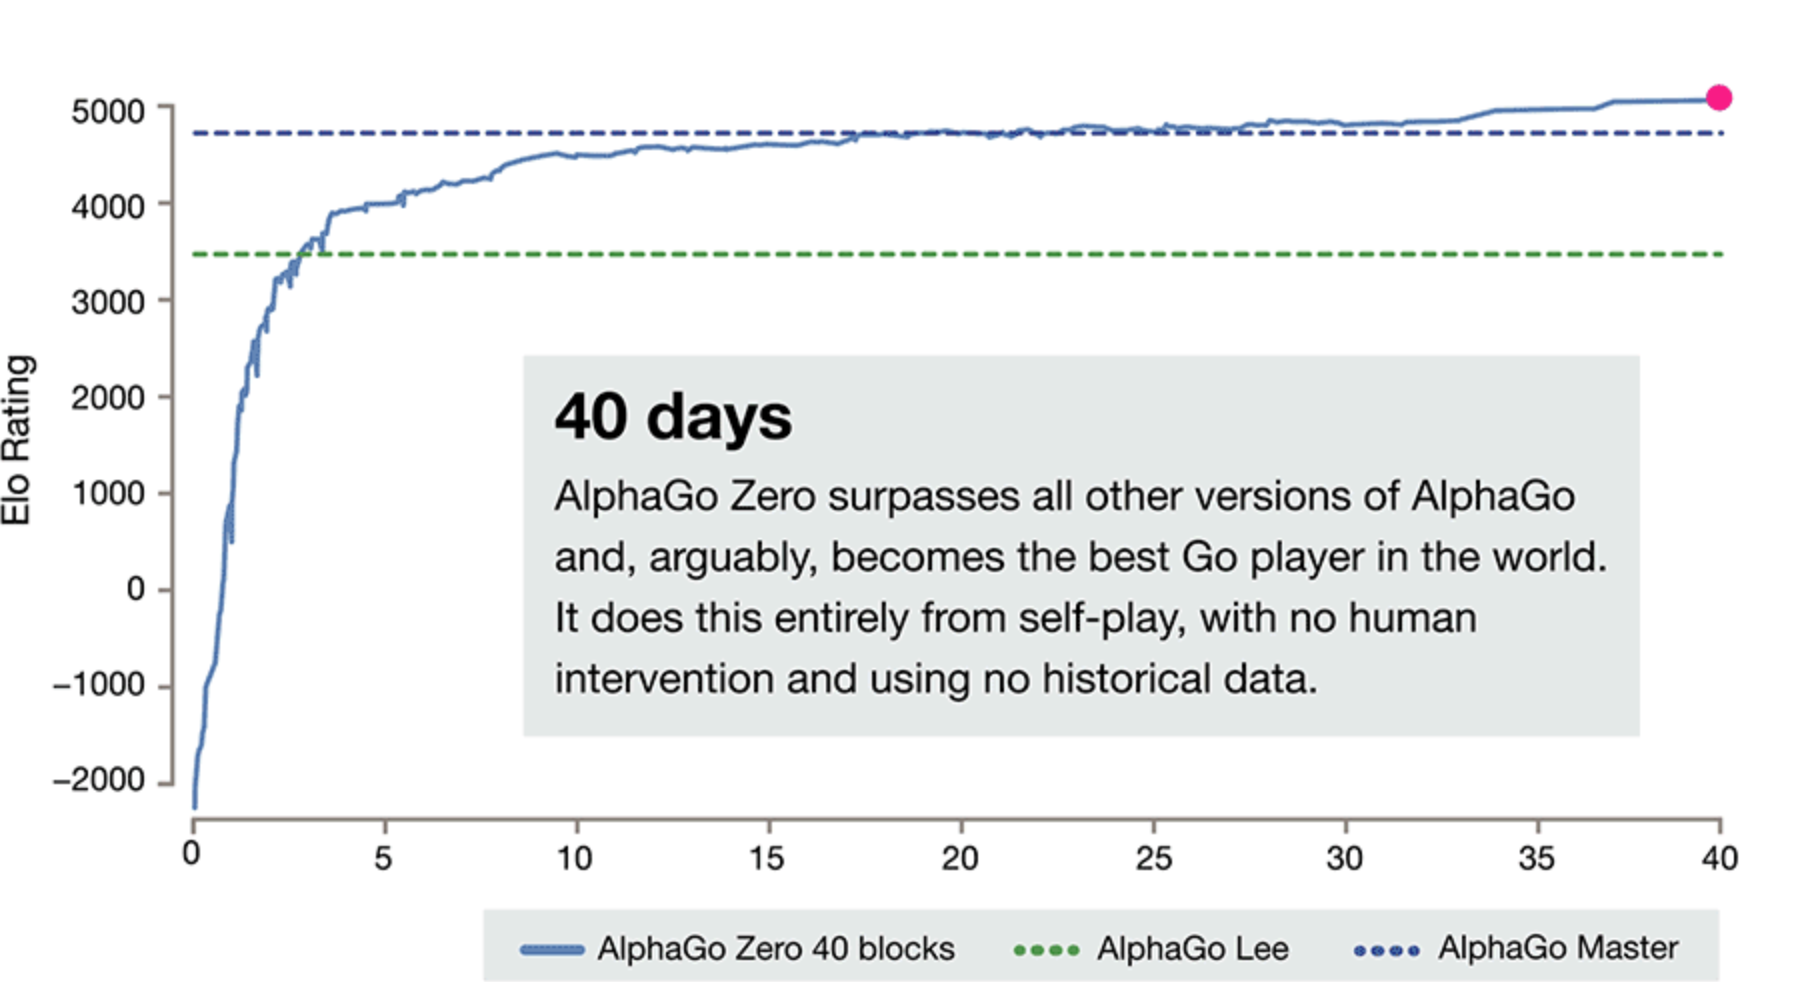
\includegraphics[width=1.1\textwidth]{figures/rl/alphago_zero.png}
		\caption{AlphaGo Zero Training Time}
		\label{fig:alphago_train}
	\end{subfigure}
	\hfill
	\begin{subfigure}[b]{0.4\textwidth}
		\centering
		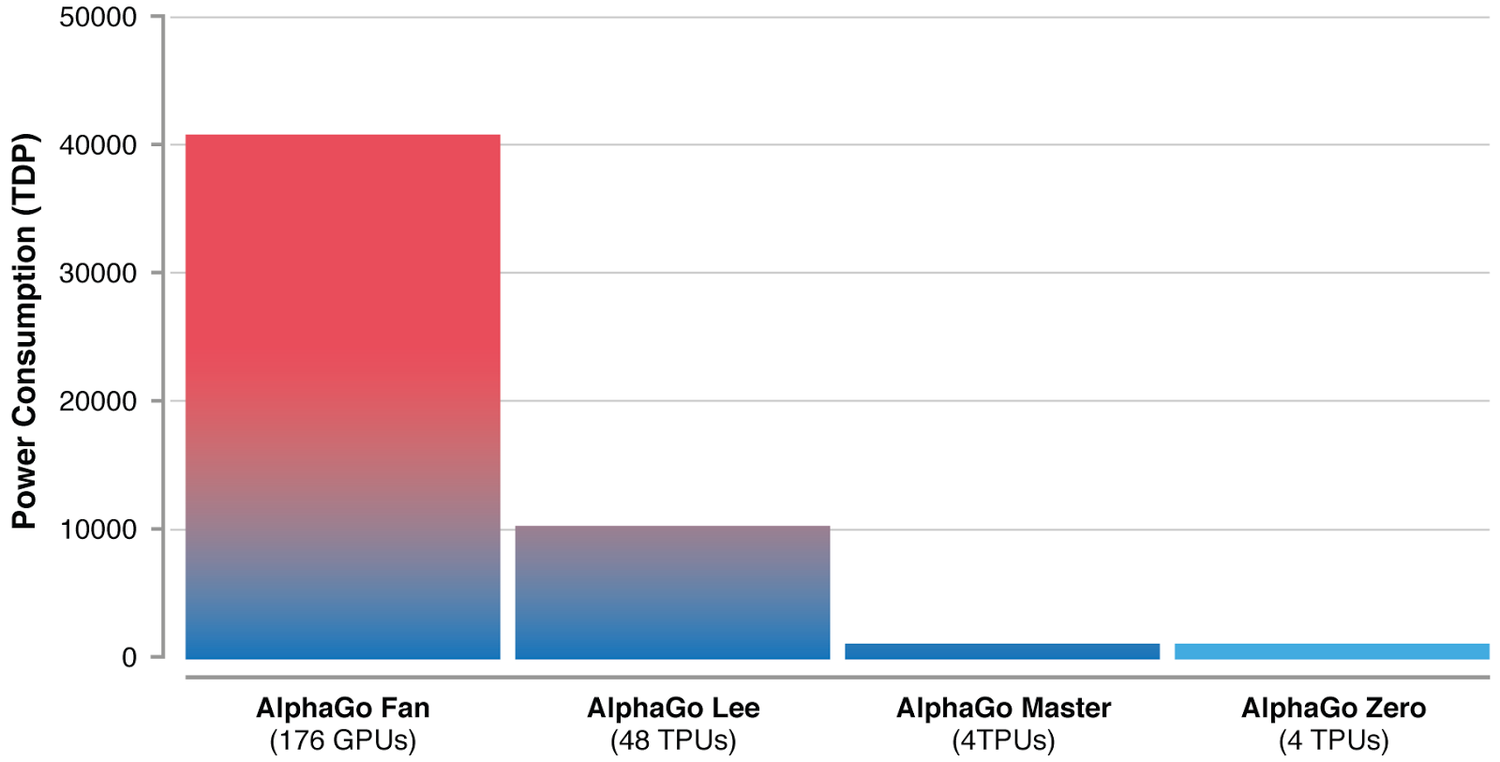
\includegraphics[width=1.1\textwidth]{figures/rl/alphago_power.png}
		\caption{AlphaGo Versions Compute Power}
		\label{fig:alphago_power}
	\end{subfigure}
	\hfill
	
	\begin{subfigure}[b]{0.4\textwidth}
		\centering
		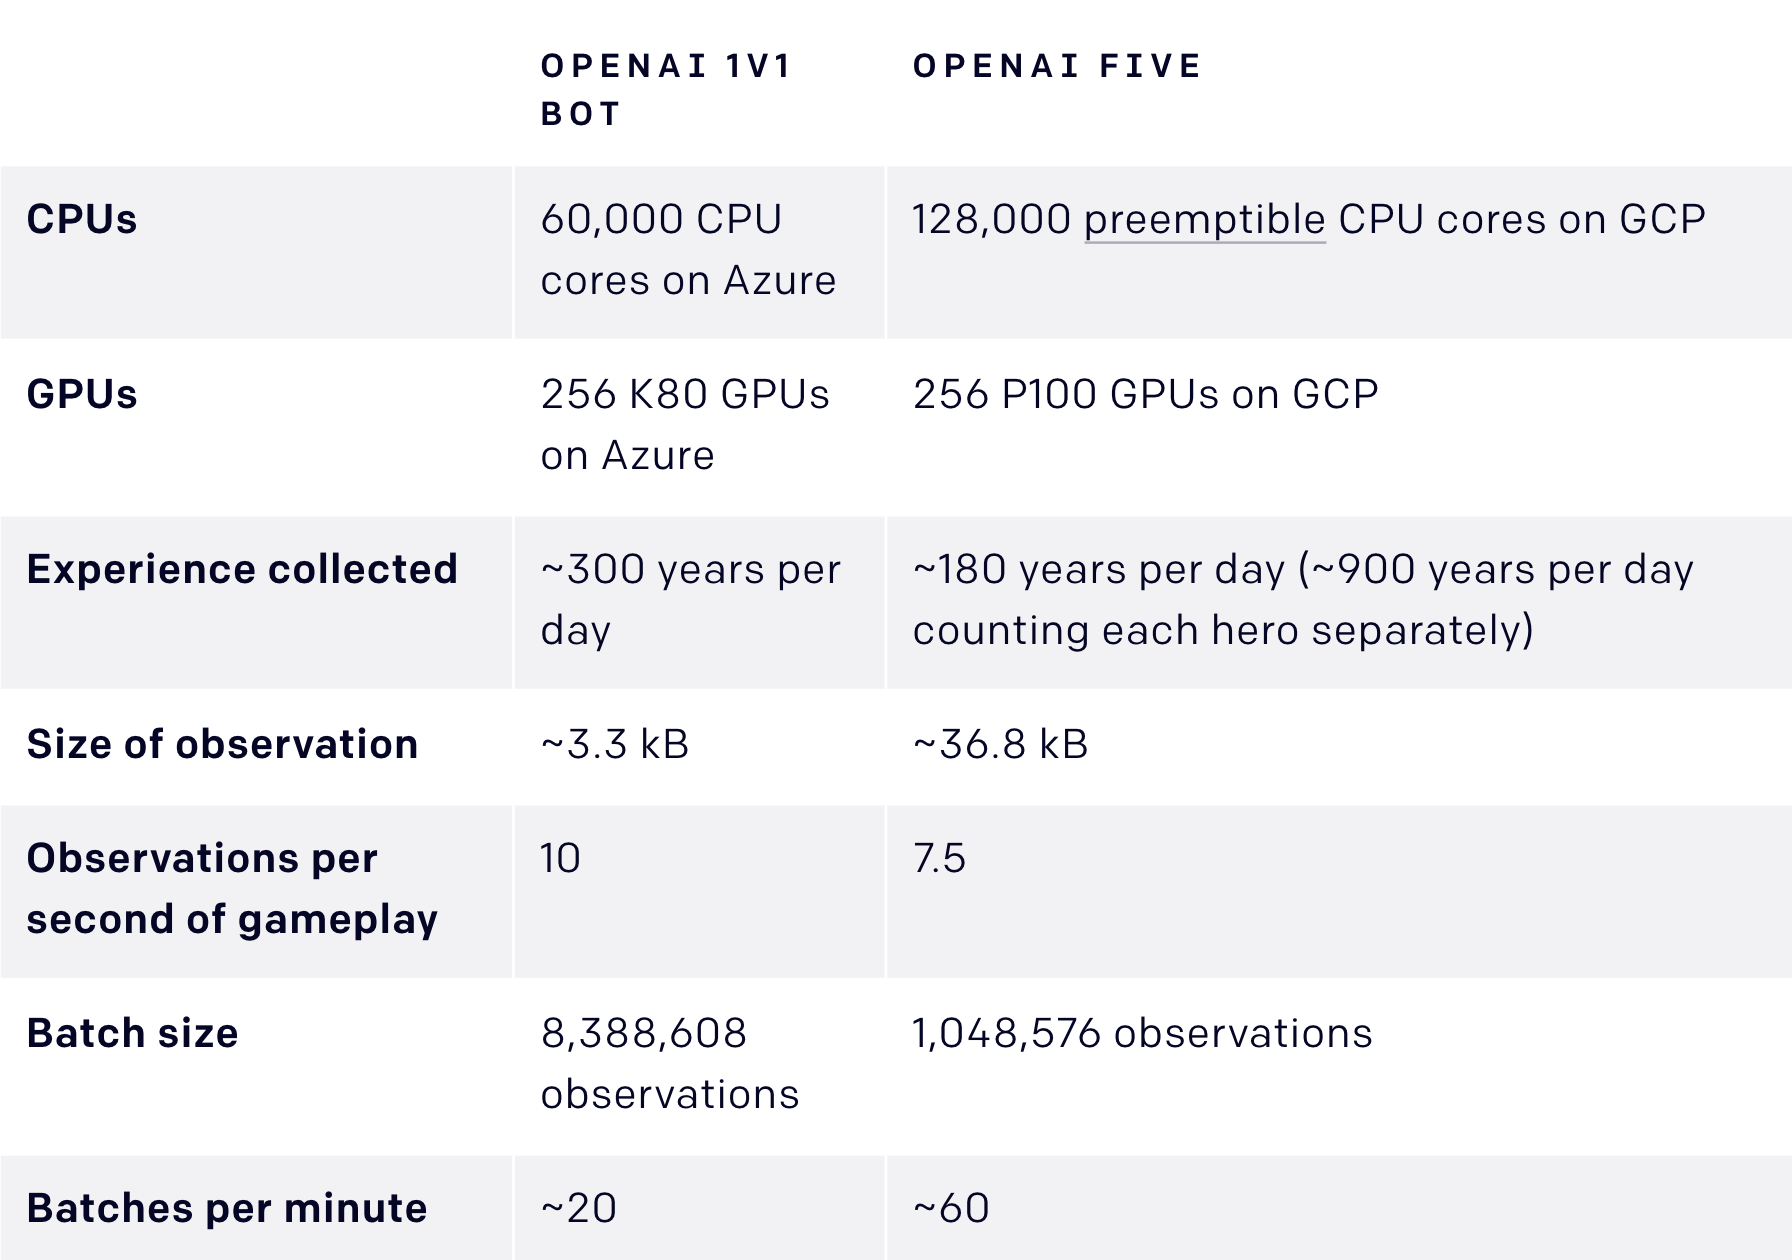
\includegraphics[width=1.1\textwidth]{figures/rl/openai_five_hardware.png}
		\caption{Hardware used for OpenAI Five}
		\label{fig:five_hardware}
	\end{subfigure}
	\hfill
	\begin{subfigure}[b]{0.4\textwidth}
		\centering
		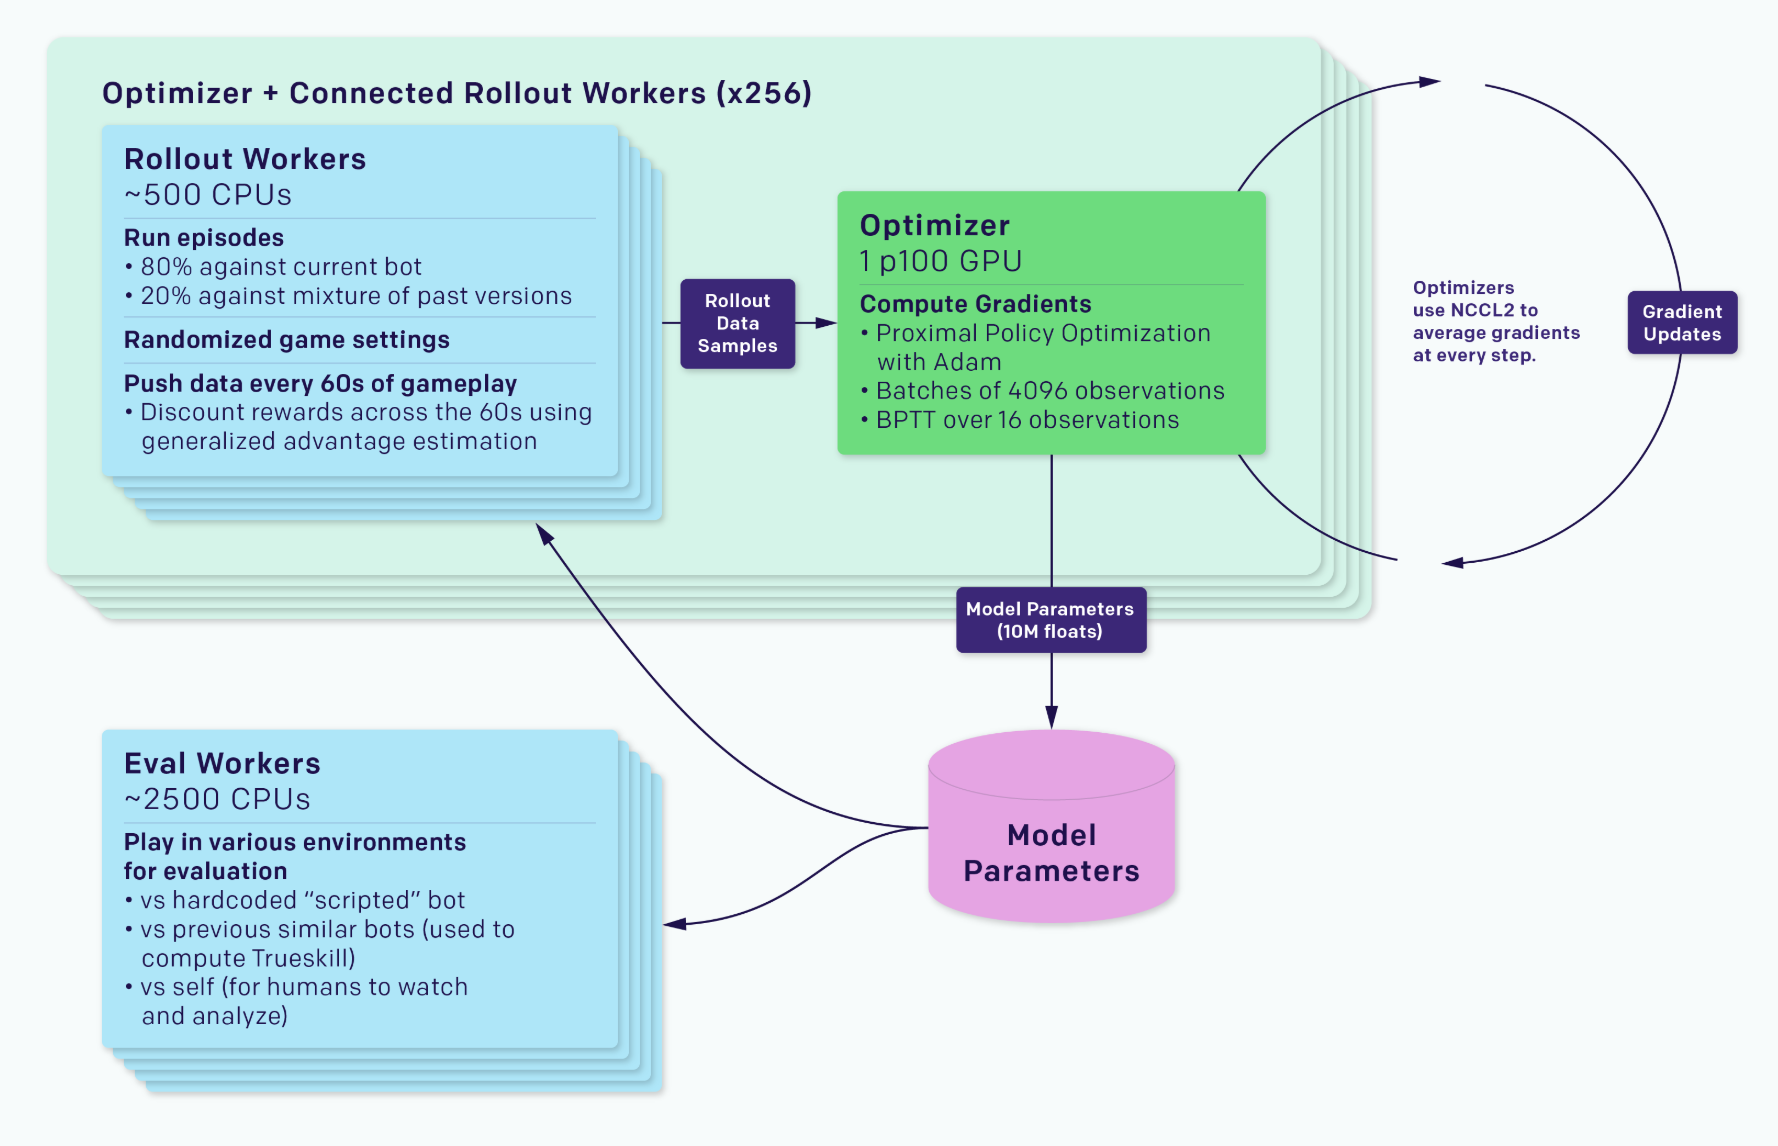
\includegraphics[width=1.1\textwidth]{figures/rl/openai_five_training.png}
		\caption{OpenAI Training Workflow}
		\label{fig:openai_five_training}
	\end{subfigure}
	\hfill
	\caption[AlphaGo Zero \& OpenAI Five]{AlphaGo Zero \& OpenAI Five (Architecture and Training Time)\protect\footnotemark}
	% \caption{AlphaGo Zero \& OpenAI Five}
	\label{fig:zero_and_five}
\end{figure}

\footnotetext{\label{alhpa_five}The Figures are from \url{https://deepmind.com/blog/alphago-zero-learning-scratch/}\\ and \url{https://openai.com/five/}}

This introduces a critical \textit{\textbf{(experiment turn-around time)}} bottleneck for RL research. Another key issue to design algorithms that are both scalable and data-efficient. To overcome these bottlenecks, new approaches and directions are followed towards using distributed setups to accelerate RL experiments, reduce the training time, and scales the algorithms effectively. This means RL needs to support fine-grained computations and render actions in milliseconds when interacting with the real world or performing vast numbers of simulations. It has to support utilizing the resources usage and support heterogeneity in time for both simulation time which takes milliseconds or hours and the GPUs and CPUs wall-time for simulations. Also, supporting dynamic execution, as results of simulations or interactions with the environment can change future computations. 

This leads the way to build new frameworks and investigate how to optimize existing RL algorithms for modern computers. This enables a better usage of multiple CPUs and GPUs and the combination between them, providing the proper scalability and utilizing distributed training.

Recently, there have been a quite interest and research on the scalability and distribution of RL algorithms and training with parallel environments to enhance the performance of the agents and reduce the amount of time it takes to master the learning task.

\section{Objectives}
In this research project, the aim is to train and test a set of reinforcement learning algorithms in different RL environments. The experiments are performed in non-distributed setup \& in a parallel and distributed setup. This allows to measure the effect on the training process and compare the performance among these experiments. Hence, showing the effect of the distribution and the power of using and utilizing multiple CPUs and GPUs setup. 

We will compare the state of the art algorithms mentions in the related work in Section~\ref{related_work} using Ray framework as our backend framework for the experiments along with some of the implemented algorithms. We have created our abstract class to unify the differences between RL environments methods providing simplicity and clarity.

Then with our distributed learning architecture and setup we provide evaluation for distribution and transferability of networks between different physics simulators with full benchmarking for all the experiments we have done along with comparisons between all of the environments and algorithms.

\section{Overview and Outline}
The work is organized as follows. In Chapter~\ref{chapter:background_and_foundations}, the theoretical background linked to reinforcement learning and the Markov decision process framework are introduced. Furthermore, we discuss the use of deep learning in the RL framework and the state of the art algorithms. Finally, we discuss the related work and existing distributed framework. Chapter~\ref{chapter:methodology} presents the task description, the setup of our experiments with the architecture, frameworks, and classes used to accomplish our research goal. Chapter~\ref{chapter:experiments} is a full description for all the experiments we have done along with the results and comparisons. Finally, Chapter~\ref{chapter:conclusion_and_future_work} summarizes the work, discusses future work and concludes.